\section{Generating contention via CPU instructions}
\label{sec:interconnect-sc-store-ops}

There are two primary ways one can generate traffic on the PCIe link.
1) CPU \textit{load} or \textit{store} instructions on memory-mapped PCIe configuration, device memory, or I/O address space, and 
2) direct memory access (DMA) to copy data between the PCIe device memory and the DRAM.
We now discuss how to use CPU instructions to generate the traffic and defer the discussion of generating traffic via DMA to \Cref{sec:interconnect-sc-dma}.
We also answer \textbf{RQ1}, ``Is it possible to create contention in PCIe links without the adversary saturating the PCIe bandwidth?''.

An adversary can generate traffic from the CPU by mapping a PCIe device resource to an application running on the CPU and issuing load or store operations on the mapped memory.
Each load/store operation will be buffered in the PCIe controller until a transaction layer packet (TLP) is generated and ready to be transmitted.
Two factors influence the actual transmission time of the packet:
1) The ordering of the packets, as outlined in \Cref{tab:pcie-transaction-ordering-rules}, and
2) The number of pending packets in the PCIe controller buffer that are not subject to any ordering rules relative to the current packet.
Suppose the packets do not have any relative ordering rule. 
In that case, the ordering of the packets is solely dependent on the scheduling algorithm of the PCIe controller and can not be influenced by the attacker.
As such, any packet generated by the adversary can be delayed due to existing traffic in the buffer based on the controller's scheduling policy and the ordering rules.
If there is no traffic in the buffer, the adversary's packets will not be delayed.
As a result, the attacker can detect the presence or absence of victim traffic without saturating PCIe bandwidth if the PCIe controller schedules packets without ordering constraints using a first-in-first-out (FIFO) or similar policy.

To observe the victim traffic, the attacker should ensure they have a packet pending in the PCIe controller as frequently as possible.
This ensures that the attacker can observe the presence or absence of victim traffic at a fine granularity.
The attacker also needs to ensure that the packet would not be delayed because of their traffic.
To achieve these goals, the attacker must determine the correct combination of the PCIe resource and instruction, as different instructions on different resources can lead to different PCIe transactions and transaction ordering rules.


\subsection{Challenges}
\label{subsec:interconnect-sc-store-ops-challenges}


\subsubsection{Determining the right PCIe resource and instruction combination}

Of the transaction types outlined in \Cref{tab:pcie-transaction-types}, a software application can generate only configuration read and write and memory read and write on a modern system that only has PCIe devices
\footnote{I/O reads and writes may be available if a legacy PCI device is attached.
The software application does not control messages and Completions and, hence, can not be generated directly by the adversary.}.
However, as memory reads, configuration reads, and configuration writes are all non-posted transactions, they all exhibit the same behaviour.
As such, exploring only memory reads suffices for exploring all non-posted transactions.
Similarly, exploring memory writes as transactions that an attacker can use suffices to explore all posted transactions. 


To profile the execution time of memory \textit{load} and \textit{store} instructions, we use a program that follows the pseudocode outlined in \Cref{lst:pcie-mem-reads-v-writes}.
As we can see in \Cref{fig:pcie-mem-reads-v-writes}, the execution time of memory loads (and consequently, non-posted transactions) increases linearly with the number of memory loads issued.
Each \textit{load} instruction takes about 2000 cycles, which is 625ns on a processor with a base clock of 3.2GHz.
Most of the 625ns latency is composed of PCIe transfer time \cite{neugebauer2018understanding}, because a \textit{load} operation has to wait for a previous \textit{load} operation to complete 
\footnote{While this is not enforced by PCIe ordering rules, it may be enforced by the proprietary PCIe controller implementation.}.
Since each \textit{load} instruction must wait for the previous one to complete, the attacker cannot guarantee a packet is always ready in the PCIe controller for transmission when the victim is simultaneously transmitting.
However, a memory store does not have to wait for a previous store to complete.
As such, we determine that memory stores are the correct type of transaction for the attacker.


\begin{minipage}{\textwidth}
    \lstinputlisting[language=Python]{code/interconnect-sc/pcie-mem-reads-v-writes.py}
    \captionsetup{type=lstlisting}
    \caption{Profiling the execution time of \textit{load/store} instruction.
    Each instruction reads/writes 8 bytes and is issued on a memory address at an offset of 64 bytes from the previous address.}
    \label{lst:pcie-mem-reads-v-writes}
\end{minipage}

\begin{figure}[!htb]
    \centering
    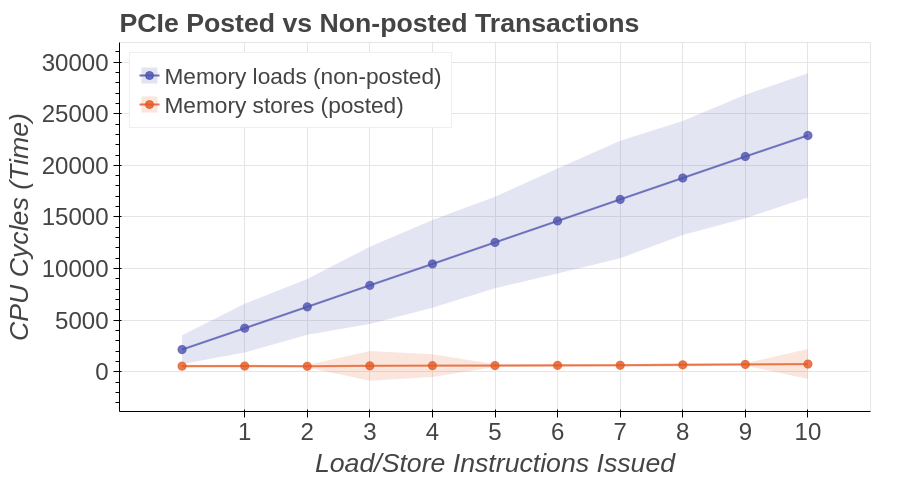
\includegraphics[width=0.8\columnwidth]{figures/interconnect-sc/store-ops/pcie_mem_reads_v_writes.png}
    \caption{Comparison: PCIe memory reads vs writes.
    The time is for completing all \textit{N} loads and stores.
    Each load needs to wait for the previous load to complete, but stores can be issued in parallel.}
    \label{fig:pcie-mem-reads-v-writes}
    % 2025-03-01_15-15
\end{figure}

\subsubsection{Issuing and timing a continuous stream of \textit{store} instructions}
\label{subsubsec:interconnect-sc-store-ops-challenges-measuring-time}

The \textit{mfence} instruction in \Cref{lst:pcie-mem-reads-v-writes} ensures prior \textit{store} operations complete before the \textit{mfence} does.
However, it disrupts the attacker from issuing a continuous stream of \textit{store} operations.
Simply removing the \textit{mfence} from the code is not sufficient, as then the end \textit{timer} may execute out of order with respect to the issued \textit{store} operations, giving a false execution time.
To fix this, the attacker needs a mechanism that can issue as many \textit{store} instructions as possible while having the ability to time the completions at the level of each instruction.

To measure the completion time of a \textit{store} operation which is issued out-of-order, we make use of two key insights:

\textit{First}, the CPU core needs to keep track of all instructions executed out-of-order so that they are retired in program order.
Keeping track of this requires a scheduler and a buffer in the hardware, which would have a limited and fixed size.
The AMD CPU has four schedulers as described in \Cref{subsubsec:interconnect-sc-background-cpu-arch-pipelines}. Each scheduler has a fixed number of instruction slots, $size_{sched}$
\footnote{AMD Zen 3 schedulers have $\sim$22-24 slots per scheduler \cite{gast2023squip}.}.
In addition, for tracking \textit{load} and \textit{store} operations that are in flight, the CPU also has a load-store queue (LSQ), with a fixed number of slots for loads ($size_{ldq} = 72$) and for stores ($size_{stq} = 64$) \cite{amd_7003_software_optimization_guide}.
Suppose the total number of pending (in flight) \textit{store} instructions is larger than the total size of the scheduler slots and the store queue. 
In that case, the next instruction will be blocked until one (or more) of the previous instructions finishes.
\textit{Second}, as the \textit{store} instructions may be executed out of program order, the attacker needs to observe the completion of the first \textit{store} instruction that was executed and not the first one by program order.
% As discussed in \Cref{subsec:interconnect-sc-background-cpu-arch}, each scheduler on the CPU core can hold 24 instructions.
% Any instruction not yet in the scheduler can not be executed out of order until it gets a slot in one of the schedulers.
% We leverage this CPU behaviour to develop a mechanism that can issue multiple \textit{store} instructions while having the ability to time individual completions.

We can use these insights to queue a \textit{timer} instruction immediately after issuing $size_{sched} + size_{stq}$ stores, and that \textit{timer} will execute only after the first \textit{store} instruction that was issued has been completed.
To achieve this, we need to ensure that we can issue $N = 3 * size_{sched} + size_{stq}$ 
\footnote{Only three schedulers have an address generation unit (AGU) that triggers \textit{load/store} operations.}
\textit{store} instructions in $t_{cpu} < 600~cycles$ (see \Cref{fig:pcie-mem-reads-v-writes}), to ensure that the CPU pipeline is filled before the first \textit{store} instruction retires.
As the AMD CPU can issue 2 \textit{store} instructions per cycle \cite{amd_7003_software_optimization_guide}, $t_{cpu} = N/2$.
For $size_{sched} = 24$ and $size_{stq} = 64$, $t_{cpu} = 68~cycles$.
As such, $t_{cpu}$ is well below the time taken for one store to complete and, hence, is sufficient to keep the CPU pipeline full.
% \footnote{Hence, if $size_{sched} = 24$, $N = 3 * 24 + 64 = 136$, and $t_{cpu} = N/2 = 68~cycles$.}.

Now, after the initial $N$ stores, if we issue a continuous stream of (\textit{timer}...\textit{store}) pairs, the \textit{timer} from the pair will be executed only after a previous \textit{store} retires.
As this \textit{timer} instruction will be executed immediately (out of order with the other stores), the \textit{store} in this pair will almost immediately occupy the now available scheduler slot, blocking the next \textit{timer}.
Thus, the difference in the results of the two \textit{timer} instructions reflects the variation in retirement times of consecutive \textit{store} instructions.
As the retirement times of the \textit{store} instructions are impacted by the PCIe transaction time, the attacker can use this mechanism to determine the presence or absence of victim traffic on PCIe.
We measure the time taken for various values of $N$ using the pseudo-code in \Cref{lst:measuring-time}
As we can see in \Cref{fig:measuring-store-time}, the measured time difference significantly increases after $N = 81$, validating this approach.

% However, we also observe that after $N = 81$, the stores retire in groups of $8$ instead of retiring individually.
% This can be an effect of some write-combining feature of the hardware.
% While the AMD CPU has a write-combining buffer immediately after the LSU, we explicitly rely on a PCIe resource marked as non-write-combining by Linux, which should prevent the hardware from relying on this buffer.


\begin{figure}[!htb]
    \centering
    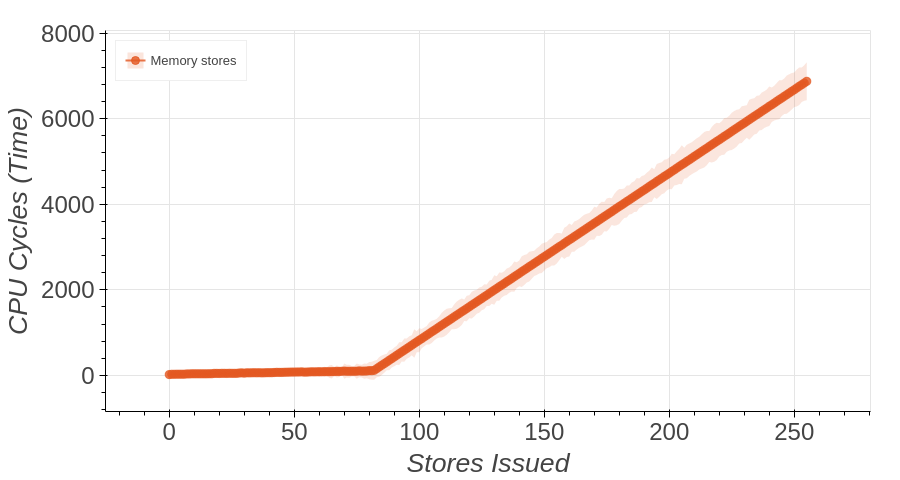
\includegraphics[width=\columnwidth]{figures/interconnect-sc/store-ops/measuring_store_time.png}
    \caption{Using head-of-line blocking in CPU pipeline to measure completion time of asynchronous stores.
    The timer is not executed out of order after a threshold number of \textit{store} instructions.}
    \label{fig:measuring-store-time}
    % 2025-03-04_15-28
\end{figure}

\begin{minipage}{\textwidth}
\lstinputlisting[language=Python]{code/interconnect-sc/measuring-time.py}
\captionsetup{type=lstlisting}
\caption{Pseudo-code for measuring time of individual stores while issuing multiple stores in parallel}
\label{lst:measuring-time}
\end{minipage}

\subsubsection{Microcode Updates}
\label{subsubsec:interconnect-sc-store-ops-challenges-microcode-updates}
However, the CPU behaviour observed in \Cref{fig:measuring-store-time} depends on the microcode the CPU is running.
The CPU microcode can change how the CPU behaves.
For example, the microcode can change how the schedulers schedule the instructions out of order, how the LSU tracks the stores in flight, or how the write-combining buffers combine multiple \textit{store} instructions to use the interconnects efficiently.

The results in \Cref{fig:measuring-store-time} are based on the microcode patch 0x0A0011D5 (for AMD EPYC 3rd gen 19h B1 processors) released on May 03, 2024 to address CVE-2023-31315 \cite{amd_microcode_update}.
Before this update (i.e. microcode patch 0x0a0011d3), the results were as shown in \Cref{fig:measuring-store-time-before-microcode-update}.
Here, $N = 120$, instead of $N = 80$. 
In addition, after the threshold of $N$, the stores complete in groups of $8$ instead of retiring individually.
This may be caused by unexpected behaviour of the write-combining (WC) buffers present after the LSU in the CPU pipeline.
The usage of the WC buffers also explains the high variation in the execution time measured, as the WC buffer combines writes based on specific threshold differences between the target addresses \cite{amd_7003_software_optimization_guide}, which are dependent on the order in which the stores were issued.
While we ensure that Linux marks the PCIe resource as a memory type that does not allow write-combining, the CPU may still use these buffers unexpectedly.
However, AMD does not offer changelogs for their microcode.
Hence, we cannot confirm what CPU behaviour changed between the given versions.


\begin{figure}[!htb]
    \centering
    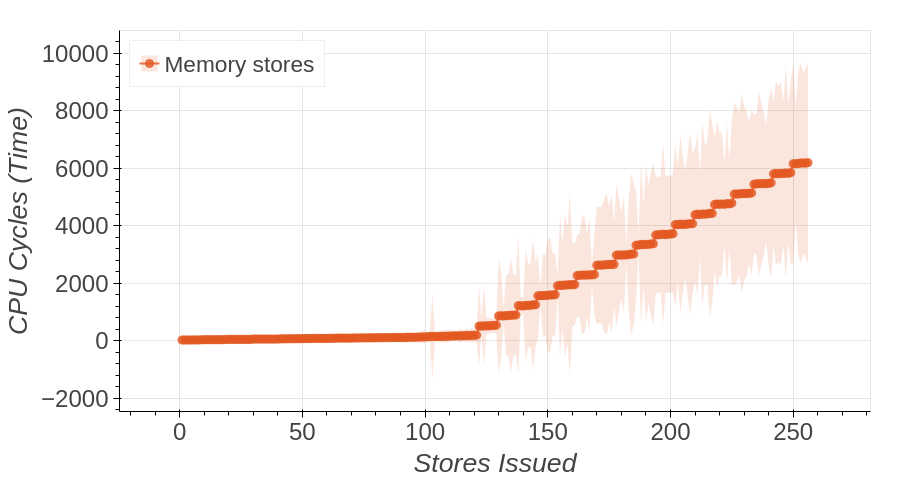
\includegraphics[width=\columnwidth]{figures/interconnect-sc/store-ops/measuring_store_time_before_microcode_update.png}
    \caption{Using head-of-line blocking in CPU pipeline to measure completion time of asynchronous stores.
    The timer is not executed out of order after a threshold number of \textit{store} instructions.}
    \label{fig:measuring-store-time-before-microcode-update}
    % 2024-10-12_18-07
\end{figure}

% \subsubsection{Reverse Engineering the CPU architecture}
% \label{subsubsec:interconnect-sc-store-ops-challenges-reverse-engineering}
\subsection{Using \textit{store} operations to observe presence/absence of victim traffic on PCIe}
\label{subsec:interconnect-sc-store-ops-measuring-time}
Now, we have a mechanism to issue multiple \textit{store} instructions in parallel while timing the completion of an individual (or a small group of) \textit{store} instructions.
We can use this mechanism along with the threshold of $N = 81$ to observe the presence or absence of victim traffic in the PCIe controller.
To achieve this, we execute the pseudo-code outlined in \Cref{lst:timing-victim-with-stores} while the victim transfers a large amount of data to or from the GPU via DMA
\footnote{Since most GPU-based applications rely on the DMA controller for efficient transfers, we assume that the victim uses DMA.}.

To evaluate our ability to detect victim traffic, we run the adversary for $10^5$ iterations.
At the same time, we execute the victim, which repeatedly (for $10^4$ iterations) performs a DMA transfer of either 4KB or 4MB.
The 4KB transfer does not saturate the PCIe link, while the 4MB transfer saturates the PCIe link (see \Cref{fig:bw-util-and-time-per-size}).
Additionally, we synchronise the execution of the critical code sections responsible for data transfers between the victim and the adversary. 
This synchronisation allows us to measure whether we can detect the presence or absence of victim traffic, even though such perfect alignment is unrealistic for a side-channel attack.

As shown in \Cref{fig:cpu-store-victim-observation}, the execution time of the individual \textit{store} operations by the adversary increases in the presence of victim traffic, irrespective of whether the victim is saturating the PCIe link or not.
In the absence of a victim, the \textit{store} instruction takes $<15~cycles$ to complete. However, in the presence of victim traffic, the execution time increases to $>15~cycles$ and drops down again once the victim is done transmitting.
As such, an adversary is able to determine the presence/absence of victim traffic.
The adversary observes a fixed delay in the execution time of the \textit{store} instruction irrespective of the size being transferred.
However, the duration for which the adversary observes the delay increases with the amount of data the victim transfers.
This is the case because the victim transfers the data using \textit{burst mode} of transfer, where the burst size is fixed.


\begin{minipage}{\textwidth}
    \lstinputlisting[language=Python]{code/interconnect-sc/timing-victim-with-stores.py}
    \captionsetup{type=lstlisting}
    \caption{Attacker code to detect presence of victim traffic via \textit{store} instructions}
    \label{lst:timing-victim-with-stores}
\end{minipage}

\begin{figure}[!htb]
    \centering
    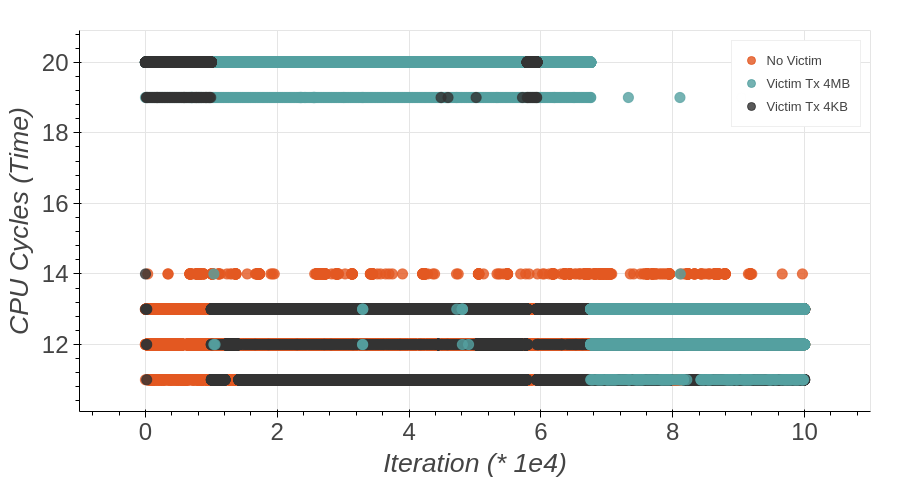
\includegraphics[width=\columnwidth]{figures/interconnect-sc/store-ops/cpu_store_victim_observation.png}
    \caption{Observing the presence of victim DMA traffic using \textit{store} instructions. The victim does $10^4$ iterations of transferring 4KB/4MB.}
    \label{fig:cpu-store-victim-observation}
    % 2025-03-06_14-20
\end{figure}

% \subsection{Evaluation}
\label{subsec:interconnect-sc-store-ops-evaluation}
